\documentclass{beamer}

%================================================
% THEME AND PACKAGES
%================================================

\usetheme{Madrid}

\usepackage{graphicx}
\usepackage{booktabs}
\usepackage{array}
\usepackage{ragged2e}
\usepackage{xcolor}
\usepackage{tikz}

% TikZ positioning library
\usetikzlibrary{positioning}

%================================================
% COLORS
%================================================

\definecolor{EcoGreen}{RGB}{62,207,142}
\definecolor{DarkGreen}{RGB}{20,100,70}

\setbeamercolor{structure}{fg=DarkGreen}
\setbeamercolor{frametitle}{fg=DarkGreen}

%================================================
% FRAME TITLE
%================================================

% Make every slide title clearly visible
\setbeamertemplate{frametitle}{%
    \vspace{0.2cm}
    \noindent
    {\color{DarkGreen}\Large\bfseries\insertframetitle}
    \par
    \vspace{0.2cm}
}

%================================================
% PRESENTATION INFORMATION
%================================================

\title{\textbf{ECOLOOP}}
\subtitle{A Smart Campus Electronics Reuse, Component Harvesting \& Repair Platform}

\author{}
\institute{M.Tech CSE, ECE\\
\vspace{0.2cm}
NSS College of Engineering, Palakkad}

\date{}

%================================================
% DOCUMENT
%================================================

\begin{document}

%================================================
% SLIDE 1: TITLE SLIDE
%================================================

\begin{frame}
    \titlepage
\end{frame}

%================================================
% SLIDE 2: INTRODUCTION
%================================================

\begin{frame}{Introduction}

\begin{itemize}
    \item Electronic waste and abandoned components are a continuous challenge in engineering colleges.

    \item Student academic projects and syllabus upgrades leave behind functional boards, sensors, and peripherals.

    \item Usable microcontrollers and ICs are frequently left idle or discarded after semester evaluations.

    \item Junior students repeatedly purchase the exact same components from retail markets at high costs.

    \item \textbf{EcoLoop} establishes a closed-loop, peer-to-peer circular economy platform designed specifically for the NSSCE campus.
\end{itemize}

\end{frame}

%================================================
% SLIDE 3: PROBLEM STATEMENT
%================================================

\begin{frame}{Problem Statement}

\begin{block}{Challenges in Campus Hardware Utilization}

\begin{itemize}
    \item \textbf{Component Dormancy:} Functional electronic components sit unused in hostel rooms and lockers after project completions.

    \item \textbf{Lack of a Campus Exchange Channel:} No dedicated, verified platform exists for students to discover surplus hardware across departments.

    \item \textbf{Unnecessary Student Expenditure:} Students spend thousands of rupees each semester buying hardware already available on campus.

    \item \textbf{Premature Disposal:} Slightly malfunctioning hardware is discarded rather than diagnosed or repaired.

    \item \textbf{Trust \& Verification Gap:} Open marketplace channels suffer from unverified claims and unreliable handoffs.
\end{itemize}

\end{block}

\end{frame}

%================================================
% SLIDE 4: PROPOSED SOLUTION
%================================================

\begin{frame}{Proposed Solution}

\begin{columns}

\column{0.32\textwidth}

\begin{block}{Circular Marketplace}

\centering

\textbf{Peer Exchange}

\vspace{0.1cm}

Branch-filtered hardware exchange with ₹0 gifting and component harvesting.

\end{block}

\column{0.32\textwidth}

\begin{block}{AI Hardware Scanner}

\centering

\textbf{Gemini 2.5 Vision}

\vspace{0.1cm}

Instant camera-based hardware recognition, materials detection, and risk assessment.

\end{block}

\column{0.32\textwidth}

\begin{block}{Peer Repair Platform}

\centering

\textbf{Collaborative Fixes}

\vspace{0.1cm}

AI-guided diagnostics paired with a public peer-to-peer campus troubleshooting feed.

\end{block}

\end{columns}

\vspace{0.3cm}

\begin{center}
\textbf{Secured by NSSCE Institutional Google Auth \& Dynamic QR Code Verification}
\end{center}

\end{frame}

%================================================
% SLIDE 5: OBJECTIVES
%================================================

\begin{frame}{Objectives}

\begin{itemize}

    \item Enable a peer-to-peer electronics reuse network across all engineering departments.

    \item Introduce \textbf{Component Harvesting} to salvage sub-assemblies (screens, sensors, modules) from complex or dead devices.

    \item Deploy AI computer vision to automatically categorize hardware and identify safety hazards.

    \item Establish a collaborative campus repair culture to inspect and fix hardware before discarding.

    \item Enforce institutional trust through official \texttt{@nssce.ac.in} domain-restricted access.

    \item Implement double-blind physical meetup verification using dynamic QR codes and secure 4-digit PINs.

    \item Ensure high-speed responsiveness with sub-millisecond in-memory caching and client-side image compression.

\end{itemize}

\end{frame}

%================================================
% SLIDE 6: MAJOR MODULES
%================================================

\begin{frame}{Major Modules}

\begin{center}

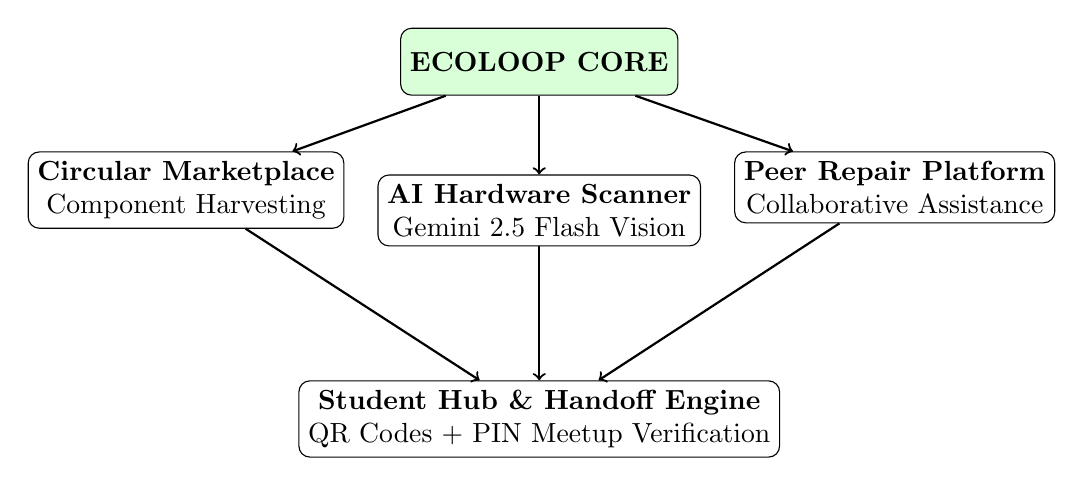
\begin{tikzpicture}[
    node distance=1.0cm,
    every node/.style={
        draw,
        rounded corners,
        align=center,
        minimum width=3.2cm,
        minimum height=0.85cm
    }
]

\node (eco) [fill=green!15]
{\textbf{ECOLOOP CORE}};

\node (market) [below left=of eco]
{\textbf{Circular Marketplace}\\Component Harvesting};

\node (ai) [below=of eco]
{\textbf{AI Hardware Scanner}\\Gemini 2.5 Flash Vision};

\node (repair) [below right=of eco]
{\textbf{Peer Repair Platform}\\Collaborative Assistance};

\node (hub) [below=1.7cm of ai]
{\textbf{Student Hub \& Handoff Engine}\\QR Codes + PIN Meetup Verification};

\draw[->,thick] (eco) -- (market);
\draw[->,thick] (eco) -- (ai);
\draw[->,thick] (eco) -- (repair);

\draw[->,thick] (market) -- (hub);
\draw[->,thick] (ai) -- (hub);
\draw[->,thick] (repair) -- (hub);

\end{tikzpicture}

\end{center}

\end{frame}

%================================================
% SLIDE 7: CIRCULAR ELECTRONICS MARKETPLACE
%================================================

\begin{frame}{Circular Electronics Marketplace}

\textbf{Purpose:} Enable engineering students to exchange and acquire hardware within the campus.

\vspace{0.2cm}

\begin{itemize}

    \item \textbf{Branch-Level Filtering:} Real-time dynamic counts across all 6 departments (CSE, ECE, EEE, Mechanical, Civil, IC).

    \item \textbf{Flexible Pricing Options:}
    \begin{itemize}
        \item \textbf{Free Surplus Gifts (₹0):} Donated items to support junior student projects.
        \item \textbf{Priced Hardware:} Subsidized peer-to-peer student rates.
    \end{itemize}

    \item \textbf{Component Splitting Support:} Sellers can list harvestable sub-assemblies alongside the main unit.

    \item \textbf{Custom Meetup Locations:} Buyers specify exact campus meeting spots (e.g., \textit{``Outside CSE Lab 204''}, \textit{``Canteen Table 4''}) upon reservation.

\end{itemize}

\end{frame}

%================================================
% SLIDE 8: DUAL-VERIFICATION HANDOFF PROTOCOL
%================================================

\begin{frame}{Dual-Verification Handoff Protocol}

\begin{enumerate}

    \item \textbf{Listing:} Student A lists a component or hardware module.

    \item \textbf{Claim:} Student B reserves the item and designates a campus meetup spot.

    \item \textbf{Token Generation:} System generates a unique 4-digit PIN and dynamic QR code for Student B.

    \item \textbf{Physical Meetup:} Both students meet at the designated campus location.

    \item \textbf{Inspection:} Student B physically tests and inspects the hardware.

    \item \textbf{Verification:} Student B presents the QR code or 4-digit PIN to Student A.

    \item \textbf{Completion:} Student A enters the code on their dashboard; the item is marked as verified and sold.

\end{enumerate}

\vspace{0.2cm}

\begin{alertblock}{Security Benefit}
Completely eliminates unverified claims, ghost reservations, and disputes over hardware delivery.
\end{alertblock}

\end{frame}

%================================================
% SLIDE 9: AI HARDWARE SCANNER
%================================================

\begin{frame}{AI Hardware Scanner}

\textbf{Technology:} Google Gemini 2.5 Flash Vision Multimodal Model

\vspace{0.2cm}

Students capture a live photo or upload an image of unknown/discarded electronics directly from their phone or laptop.

\vspace{0.2cm}

\textbf{Automated AI Vision Extraction:}

\begin{itemize}

    \item \textbf{Hardware Identification:} Identifies exact board models, microcontrollers, and IC types.

    \item \textbf{Hardware Category:} Classifies into Sensors, Embedded Systems, Displays, Peripherals, etc.

    \item \textbf{Materials Detection:} Recognizes silicon, copper traces, lithium cells, lead, and plastics.

    \item \textbf{Hazard Assessment:} Detects swollen battery risks, exposed capacitors, or toxic elements.

    \item \textbf{Action Recommendation:} Guides the user toward direct reuse, peer repair, or harvesting.

\end{itemize}

\end{frame}

%================================================
% SLIDE 10: AI SCANNER PROCESSING FLOW
%================================================

\begin{frame}{AI Scanner Processing Flow}

\begin{center}

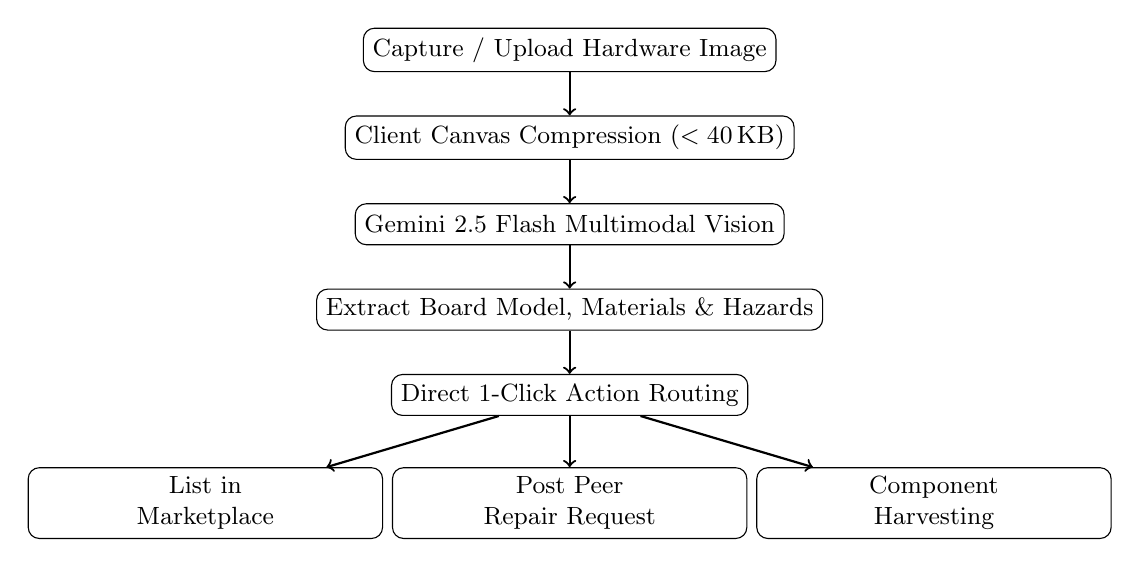
\begin{tikzpicture}[
    node distance=0.55cm,
    every node/.style={
        draw,
        rounded corners,
        align=center,
        minimum width=4.5cm,
        minimum height=0.52cm,
        font=\small
    }
]

\node (upload)
{Capture / Upload Hardware Image};

\node (compress) [below=of upload]
{Client Canvas Compression ($<40$\,KB)};

\node (gemini) [below=of compress]
{Gemini 2.5 Flash Multimodal Vision};

\node (identify) [below=of gemini]
{Extract Board Model, Materials \& Hazards};

\node (action) [below=of identify]
{Direct 1-Click Action Routing};

\node (reuse)
[below left=0.65cm and 0.1cm of action]
{List in\\Marketplace};

\node (repair)
[below=0.65cm of action]
{Post Peer\\Repair Request};

\node (salvage)
[below right=0.65cm and 0.1cm of action]
{Component\\Harvesting};

\draw[->,thick] (upload) -- (compress);
\draw[->,thick] (compress) -- (gemini);
\draw[->,thick] (gemini) -- (identify);
\draw[->,thick] (identify) -- (action);

\draw[->,thick] (action) -- (reuse);
\draw[->,thick] (action) -- (repair);
\draw[->,thick] (action) -- (salvage);

\end{tikzpicture}

\end{center}

\end{frame}

%================================================
% SLIDE 11: COMPONENT HARVESTING ARCHITECTURE
%================================================

\begin{frame}{Component Harvesting Architecture}

\textbf{The Concept:} Many discarded devices only have a single failed subsystem, while the remaining parts are completely healthy.

\vspace{0.2cm}

\begin{block}{Granular Salvage Workflow}
\begin{itemize}
    \item \textbf{Sub-Part Decomposition:} When listing a device, students register harvestable components (e.g., \textit{Keycaps, Display Panel, Power Supply, Relays}).
    \item \textbf{Selective Claiming:} Buyers can choose to acquire the \textbf{Entire Unit} or claim a \textbf{Specific Part} for their academic mini-project.
    \item \textbf{Lifecycle Multiplier:} A single abandoned device can supply components to 3--4 different student projects instead of ending up in scrap bins.
\end{itemize}
\end{block}

\vspace{0.2cm}

\begin{exampleblock}{Practical Impact}
Prevents students from purchasing an entire ₹800 sensor kit when they only need a ₹40 replacement sensor.
\end{exampleblock}

\end{frame}

%================================================
% SLIDE 12: PEER-TO-PEER REPAIR PLATFORM
%================================================

\begin{frame}{Peer-to-Peer Repair Platform}

\textbf{Philosophy:} Repair before replacement through collaborative student troubleshooting.

\vspace{0.2cm}

\begin{itemize}

    \item \textbf{AI Diagnostic Assistant:}
    \begin{itemize}
        \item Analyzes device symptoms (e.g., \textit{``Arduino COM port not recognized''}).
        \item Outlines root-cause possibilities, inspection checklists, and testing procedures.
    \end{itemize}

    \item \textbf{Public Campus Request Feed:}
    \begin{itemize}
        \item Students post unresolved device malfunctions for campus-wide peer help.
        \item Categorized by department and laboratory context.
    \end{itemize}

    \item \textbf{Peer Solver Resolution Workflow:}
    \begin{itemize}
        \item Fellow students or lab assistants can resolve tickets.
        \item Solvers document technical fix notes and record outcomes (\textit{Peer Repaired}, \textit{Lab Fixed}, or \textit{Harvested for Parts}).
        \item Public peer attribution acknowledges student contributors.
    \end{itemize}

\end{itemize}

\end{frame}

%================================================
% SLIDE 13: PERFORMANCE ENGINEERING & SPEED
%================================================

\begin{frame}{Performance Engineering \& Optimization}

To ensure smooth operation on campus networks, EcoLoop implements a high-performance optimization architecture:

\vspace{0.2cm}

\begin{itemize}

    \item \textbf{Sub-Millisecond In-Memory Caching:}
    \begin{itemize}
        \item Custom backend \texttt{SimpleTTLCache} with mutation-triggered invalidation.
        \item Tested retrieval performance: Initial query $0.40$\,ms $\rightarrow$ Cached query $\mathbf{0.00\,ms}$.
    \end{itemize}

    \item \textbf{Client SWR Architecture:} Instantaneous, zero-latency tab switching across the dashboard, marketplace, and repair platform.

    \item \textbf{In-Browser Canvas Image Compression:} Resizes camera photos to $640\times 640$ at $0.70$ JPEG quality ($\approx 35$\,KB), avoiding megabyte database bloat.

    \item \textbf{Render Background Keep-Alive Daemon:} Proactive 9-minute interval pinging eliminates cloud free-tier cold starts.

\end{itemize}

\end{frame}

%================================================
% SLIDE 14: SYSTEM ARCHITECTURE
%================================================

\begin{frame}{System Architecture}

\begin{center}

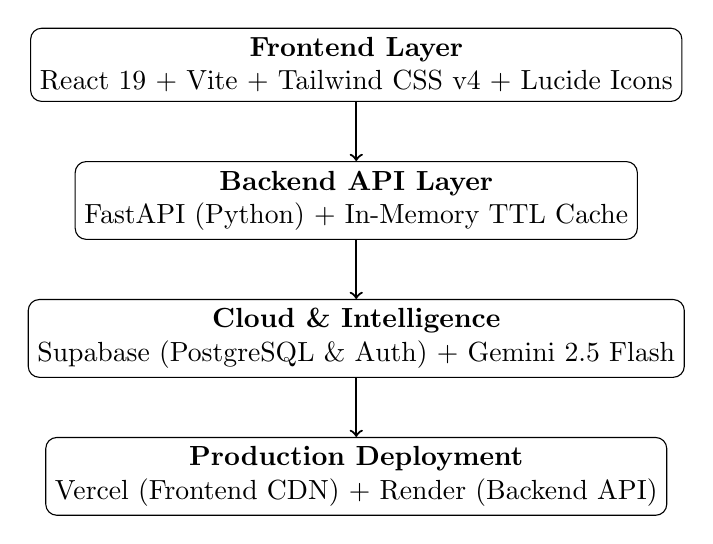
\begin{tikzpicture}[
    node distance=0.75cm,
    every node/.style={
        draw,
        rounded corners,
        align=center,
        minimum width=5.6cm,
        minimum height=0.75cm
    }
]

\node (frontend)
{\textbf{Frontend Layer}\\
React 19 + Vite + Tailwind CSS v4 + Lucide Icons};

\node (backend) [below=of frontend]
{\textbf{Backend API Layer}\\
FastAPI (Python) + In-Memory TTL Cache};

\node (cloud) [below=of backend]
{\textbf{Cloud \& Intelligence}\\
Supabase (PostgreSQL \& Auth) + Gemini 2.5 Flash};

\node (deploy) [below=of cloud]
{\textbf{Production Deployment}\\
Vercel (Frontend CDN) + Render (Backend API)};

\draw[->,thick] (frontend) -- (backend);
\draw[->,thick] (backend) -- (cloud);
\draw[->,thick] (cloud) -- (deploy);

\end{tikzpicture}

\end{center}

\end{frame}

%================================================
% SLIDE 15: DATABASE DESIGN
%================================================

\begin{frame}{Database Design}

\begin{itemize}

    \item \textbf{PROFILES}
    \begin{itemize}
        \item User UUID, authenticated email, full name, assigned department, and role.
    \end{itemize}

    \item \textbf{CIRCULAR\_ITEMS}
    \begin{itemize}
        \item Item ID, title, description, category, engineering department, price type (free/priced), price amount, condition, sub-components JSON, image URL, seller ID, buyer ID, meeting point, handoff PIN, and status (\textit{available, reserved, sold}).
    \end{itemize}

    \item \textbf{REPAIR\_TICKETS}
    \begin{itemize}
        \item Ticket ID, device name, malfunction symptoms, department, lab affiliation, AI diagnostic hints, status (\textit{open, resolved}), posted by, resolved by, and resolution notes.
    \end{itemize}

\end{itemize}

\end{frame}

%================================================
% SLIDE 16: SECURITY & INSTITUTIONAL ACCESS
%================================================

\begin{frame}{Security \& Institutional Access}

\begin{columns}

\column{0.48\textwidth}

\begin{block}{Campus Domain Authentication}

\begin{itemize}

    \item Restricted exclusively to official \textbf{\texttt{@nssce.ac.in}} Google OAuth credentials.
    \item External or personal emails are blocked at login.
    \item Mandatory onboarding assigns students to their legitimate engineering department.

\end{itemize}

\end{block}

\column{0.48\textwidth}

\begin{block}{Double-Blind Physical Trust}

\begin{itemize}

    \item Cryptographic 4-digit PIN generated uniquely per reservation.
    \item Dynamic QR code verified in person by the seller.
    \item Prevents unauthorized claims and confirms physical inspection of hardware.

\end{itemize}

\end{block}

\end{columns}

\end{frame}

%================================================
% SLIDE 17: TECHNOLOGY STACK
%================================================

\begin{frame}{Technology Stack}

\begin{table}

\centering
\small

\begin{tabular}{|l|l|}

\hline
\textbf{Component} & \textbf{Technology / Library} \\

\hline
Frontend Framework & React 19 (Hooks, Context API) \\

\hline
Build Tool & Vite \\

\hline
Styling & Tailwind CSS v4 (Dark Graphite Palette) \\

\hline
Icons \& Visuals & Lucide React \\

\hline
QR Code Generation & \texttt{qrcode} (Dynamic DataURL rendering) \\

\hline
Backend API & FastAPI (Asynchronous Python) \\

\hline
Database \& Auth & Supabase PostgreSQL + Supabase Campus Auth \\

\hline
Artificial Intelligence & Google Gemini 2.5 Flash Vision API \\

\hline
Hosting Platforms & Vercel (Frontend) + Render (Backend) \\

\hline

\end{tabular}

\end{table}

\end{frame}

%================================================
% SLIDE 18: KEY BENEFITS
%================================================

\begin{frame}{Key Benefits}

\begin{columns}

\column{0.32\textwidth}

\begin{block}{Environmental}

\begin{itemize}
    \item Diverts functional electronics from disposal.
    \item Extends component lifespans via selective part harvesting.
    \item Promotes campus sustainability.
\end{itemize}

\end{block}

\column{0.32\textwidth}

\begin{block}{Economic}

\begin{itemize}
    \item Free ₹0 hardware gifting between peers.
    \item Subsidized peer prices for student projects.
    \item Prevents duplicate retail purchases.
\end{itemize}

\end{block}

\column{0.32\textwidth}

\begin{block}{Educational}

\begin{itemize}
    \item Hands-on repair and diagnosis experience.
    \item Better access to hardware across all branches.
    \item Encourages practical troubleshooting skills.
\end{itemize}

\end{block}

\end{columns}

\end{frame}

%================================================
% SLIDE 19: EXPECTED IMPACT
%================================================

\begin{frame}{Expected Impact}

\begin{center}

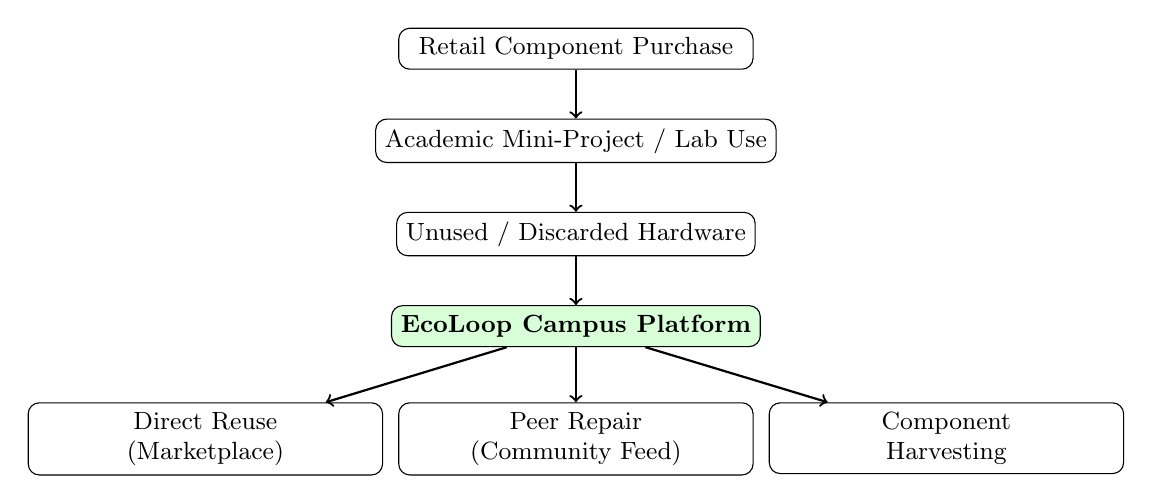
\begin{tikzpicture}[
    node distance=0.62cm,
    every node/.style={
        draw,
        rounded corners,
        align=center,
        minimum width=4.5cm,
        minimum height=0.52cm,
        font=\small
    }
]

\node (purchase) {Retail Component Purchase};

\node (use) [below=of purchase]
{Academic Mini-Project / Lab Use};

\node (unused) [below=of use]
{Unused / Discarded Hardware};

\node (eco) [below=of unused, fill=green!15]
{\textbf{EcoLoop Campus Platform}};

\node (reuse)
[below left=0.7cm and 0.1cm of eco]
{Direct Reuse\\(Marketplace)};

\node (repair)
[below=0.7cm of eco]
{Peer Repair\\(Community Feed)};

\node (salvage)
[below right=0.7cm and 0.1cm of eco]
{Component\\Harvesting};

\draw[->,thick] (purchase) -- (use);
\draw[->,thick] (use) -- (unused);
\draw[->,thick] (unused) -- (eco);

\draw[->,thick] (eco) -- (reuse);
\draw[->,thick] (eco) -- (repair);
\draw[->,thick] (eco) -- (salvage);

\end{tikzpicture}

\end{center}

\end{frame}

%================================================
% SLIDE 20: FUTURE SCOPE
%================================================

\begin{frame}{Future Scope}

Logical next-phase enhancements for the EcoLoop ecosystem:

\vspace{0.2cm}

\begin{itemize}

    \item \textbf{Smart Campus Drop-off Lockers:} Integrating physical IoT lockers with QR code scanners for asynchronous hardware exchange without scheduled meetups.

    \item \textbf{Automated Component Matching:} Notification alerts when an in-demand IC or sensor requested by a student is posted in the marketplace.

    \item \textbf{Technical Skill Endorsements:} Peer badges acknowledging students who consistently resolve hardware tickets on the repair platform.

    \item \textbf{Inter-College Extension:} Expanding verified network access across neighboring technical institutions.

\end{itemize}

\vspace{0.2cm}

\begin{alertblock}{Implementation Status}
The core Marketplace, AI Vision Scanner, Peer Repair Platform, QR Verification, and Authentication are 100\% implemented, operational, and deployed.
\end{alertblock}

\end{frame}

%================================================
% SLIDE 21: CONCLUSION
%================================================

\begin{frame}{Conclusion}

\begin{center}

{\Large \textbf{EcoLoop}}

\vspace{0.2cm}

\textbf{Circular Marketplace \quad$\bullet$\quad AI Scanner \quad$\bullet$\quad Peer Repair \quad$\bullet$\quad QR Handoffs}

\vspace{0.4cm}

\begin{block}{}

\centering
EcoLoop delivers a clean, verified, high-speed digital ecosystem that transforms discarded electronics into accessible engineering resources for NSS College of Engineering students.

\vspace{0.2cm}

By combining \textbf{AI vision identification}, \textbf{component harvesting}, and \textbf{secure physical handoffs}, the platform drastically cuts student project costs while fostering sustainable engineering practices.

\end{block}

\vspace{0.3cm}

\textbf{
Identify $\rightarrow$
Exchange $\rightarrow$
Repair $\rightarrow$
Harvest
}

\end{center}

\end{frame}

%================================================
% SLIDE 22: THANK YOU
%================================================

\begin{frame}

\begin{center}

\vspace{1.2cm}

{\Huge \textbf{THANK YOU}}

\vspace{0.6cm}

{\Large \textbf{EcoLoop}}

\vspace{0.2cm}

\textit{Smart Campus Electronics Reuse, Component Harvesting \& Repair Platform}

\vspace{0.5cm}

\textbf{NSS College of Engineering, Palakkad}

\end{center}

\end{frame}

%================================================
% END
%================================================

\end{document}
